\documentclass[ngerman, 12pt, pdftex]{scrartcl}[2006/07/30]

%encoding and input
\usepackage[ngerman]{babel} %spell correction
\usepackage[latin1]{inputenc} 
\usepackage[T1]{fontenc}

%bugfixes
\usepackage{fixltx2e} 

%Font Symbols and Colors
\usepackage{textcomp} %more symbols
\usepackage{xcolor}

%Math
\usepackage{amsmath}
\usepackage{mathtools} %extends amsmath

%Programming
\usepackage{listingsutf8} %in utf8
\lstset{language=Java,captionpos=b,tabsize=3,frame=lines,keywordstyle=\color{blue},commentstyle=\color{teal},stringstyle=\color{red},numbers=left,numberstyle=\tiny,numbersep=5pt,breaklines=true,showstringspaces=false,basicstyle=\footnotesize,emph={label},upquote=true} %Syntax highlighting

%Verbatim extension (with line numbers and tab-expansion)
\usepackage{moreverb} 

%Headers and Footer
\usepackage{fancyhdr}

%title
\title{Handbuch}
\author{Frank M\"{u}ller, Oliver Wisler, Luzius Bachmann, Fabio Sulser}
\subtitle{Swissdefcon-Team}

\begin{document}
%declare  Header
\pagestyle{fancy}
\fancyhf{} 
\fancyhead[L]{Handbuch} %left header
\fancyhead[C]{Swissdefcon-Team} %centered header
\fancyhead[R]{\thepage}  % right header
\renewcommand{\headrulewidth}{0.1pt} 	%upper separating line
%\fancyfoot[C]{\thepage} 				%centered footer, line number



%you might want to enable come features:
\maketitle
%\listoffigures 
%\listoftables


\newpage

\tableofcontents

\newpage

\section{Anmeldung}

Starte das Spiel und melde dich volgendermassen an.

\begin{figure}[h]
\centering
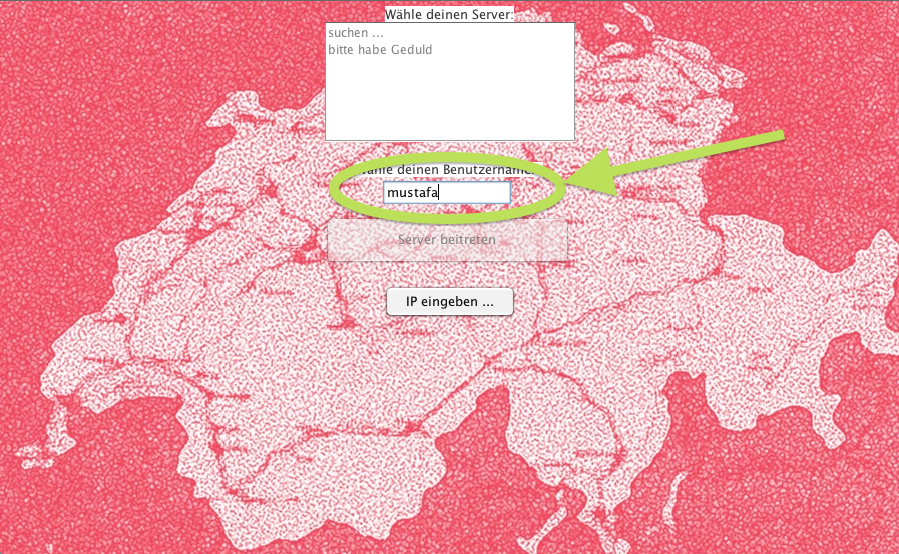
\includegraphics[scale=0.3]{starten/namen_eingeben.png}
\caption{Gib den Namen ein}
\end{figure}

Gib in dem Markierten Feld den Namen ein. Standardm\"{a}ssig wird der Name deines Computers verwendet.

\begin{figure}[h]
\centering
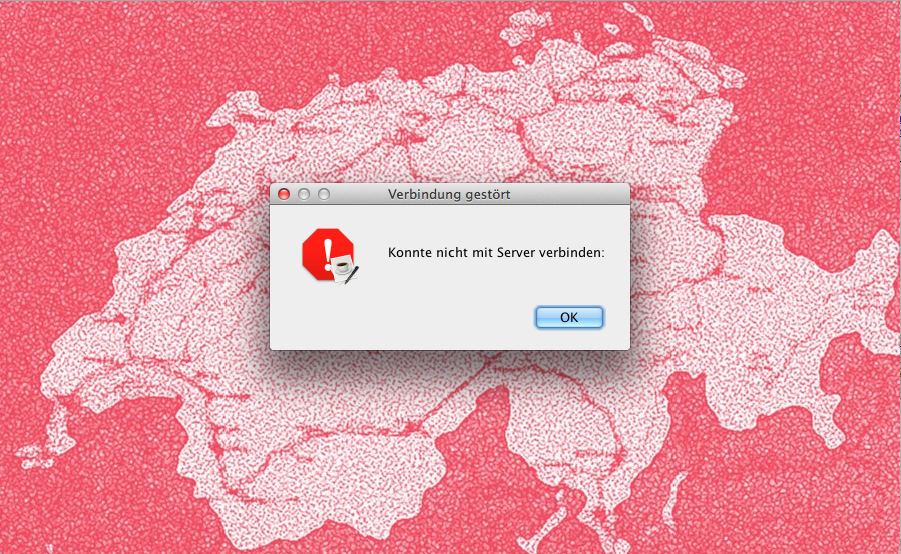
\includegraphics[scale=0.3]{starten/keine_serververbindung.png}
\caption{Error, keine Verbinfung zum Server}
\end{figure}

Falls du keine Verbindung zum Server hast wird die Obige Meldung angezeigt.

\newpage

\begin{figure}[h]
\centering
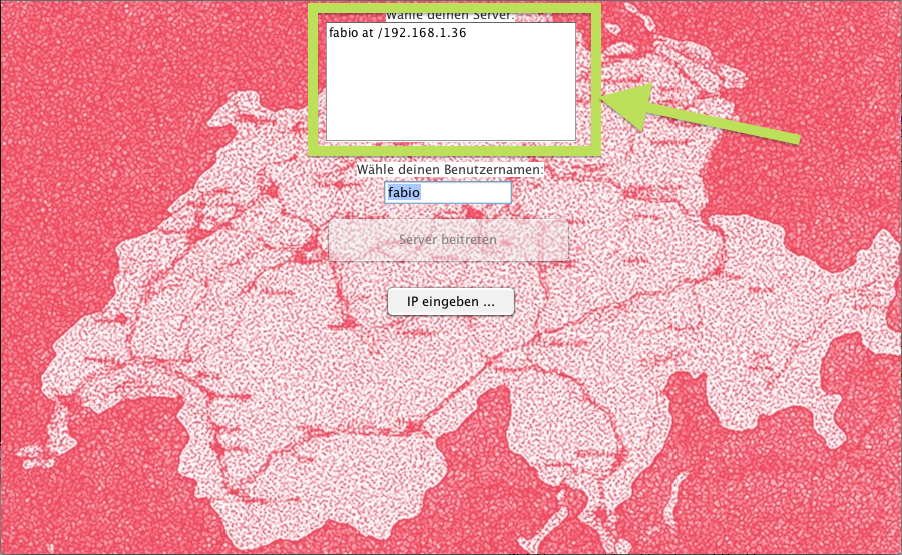
\includegraphics[scale=0.3]{starten/serverliste.png}
\caption{Liste der Server}
\end{figure}

In dem oben marierten Feld siehst du die Liste der aktiven Server.

\begin{figure}[h]
\centering
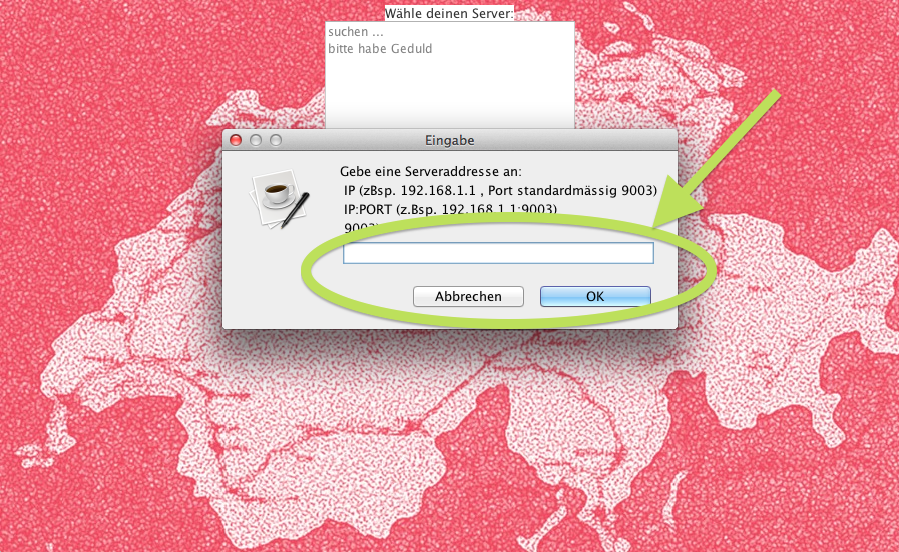
\includegraphics[scale=0.3]{starten/IP_manuell_eingeben.png}
\caption{Serveradresse eingeben}
\end{figure}

Gibt es einen Server, der nicht in der Liste angezeigt wird, so kannst du dessen Adresse auch per
Hand eingeben.

\newpage

\begin{figure}[h]
\centering
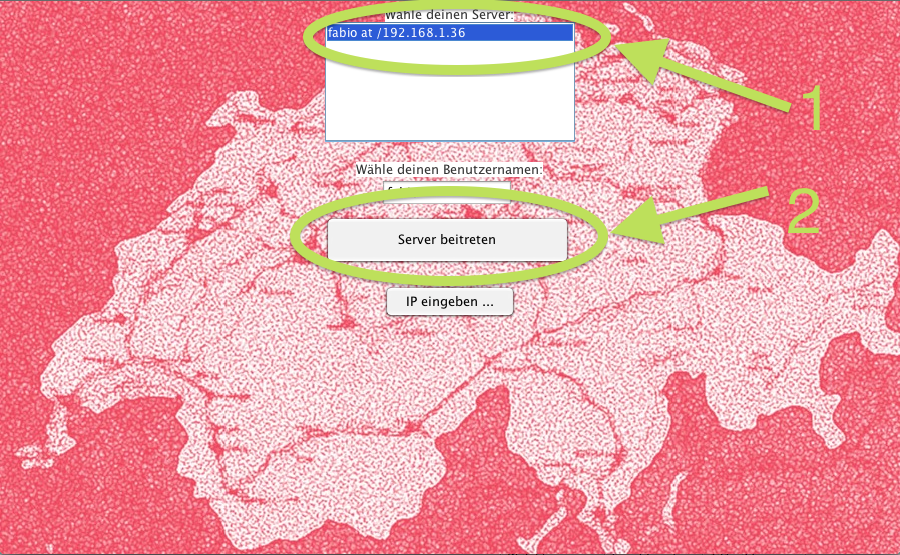
\includegraphics[scale=0.3]{starten/server_waehlen.png}
\caption{Server w\"{a}hlen}
\end{figure}

W\"{a}hle einen Server aus der ober beschriebenen Liste per Mausklick aus un gib deinen(1) und dr\"{u}cke dann auf "'Server betreten"'(2).


\newpage

\section{Lobby}

Nun hast du es geschafft und bist in der Lobby.
Auf der Rechten Seite siehst du das Chatfenster.

\begin{figure}[h]
\centering
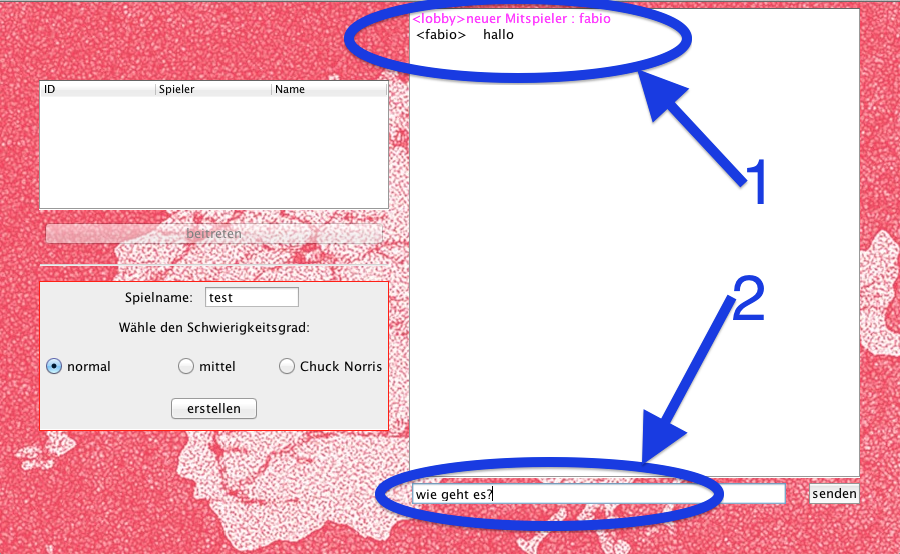
\includegraphics[scale=0.3]{lobby/chat.png}
\caption{Chat auf der Rechten Seite}
\end{figure}

In dem Chat kannst du nun Nachrichten von anderen Personen sehen, die sich auf dem selben Server wie du befinden. Zudem werden dir wichtige Informationen in dem Chatfenster angezeigt(1).
Unterhalb des Chat-Ausgabefensters siehst du das Eingabepanel, in dem du deine Nachricht eingeben kannst(2). Zum senden der Nachricht dr\"{u}cke entweder die Enter-Taste, oder dr\"{u}cke auf den senden-Button.
Eine normale Chat-eingabe ist f\"{u}r alle Mitspieler sichtbar. M\"{o}chtest du eine Private Nachricht an eine Person senden, so gieb den Befehl "'/MSG muster hallo"' in das Eingabepanel ein, wobei "'muster"' der Name des anderen Spielers ist und "'hallo"' die Nachricht, die gesendet wird.
Um deinen Nicknamen noch zu wechseln, gib den Befehl "'/VNICK muster"' in das Eingabepanel ein, wobei muster dein neuer Name ist.

\newpage

M\"{o}chtest du ein neues Spiel erstellen oder betreten, so kannst du dies Folgendermassen machen.

\begin{figure}[h]
\centering
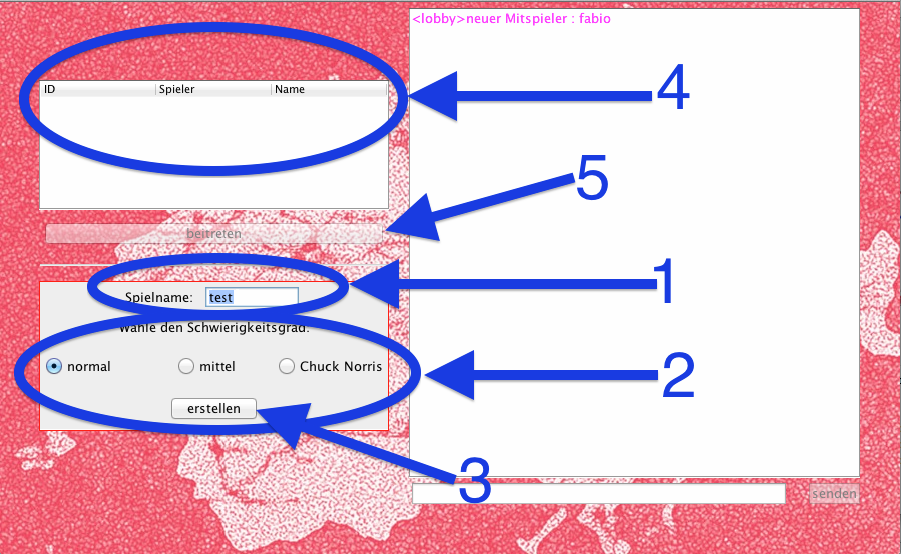
\includegraphics[scale=0.3]{lobby/spiel_erstellen.png}
\caption{Spiel erstellen oder beitreten}
\end{figure}

Um ein neues Spiel zu erstellen, so gieb im Textfeld einen neuen Spielnamen ein(1).
W\"{a}hle eine Schwierigkeitsstufe zwischen "'normal"', "'mittel"' oder "'Chuck Norris"' aus(2).
Um das erstellen des Spiels abzuschliessen dr\"{u}cke auf den Knopf erstellen.

Um einem bereits bestehenden Spiel beizutreten, so w\"{a}hle dieses per Mausklick in der Liste der Spiele (4) aus, und dr\"{u}cke dann auf den Knopf "'beitreten"'.

Danach gelangst du einen Schritt weiter. Hier siehst du einige Infos zum Spiel in dem du dich befindest.

\begin{figure}[h]
\centering
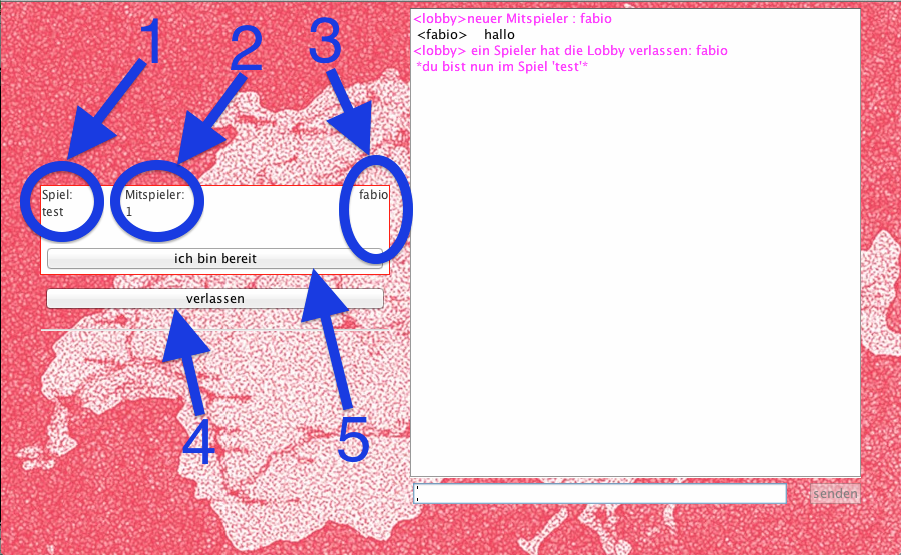
\includegraphics[scale=0.3]{lobby/spielinfos.png}
\caption{Spiel erstellen oder beitreten}
\end{figure}

 Ganz links steht der Name des Spiels(1), in der Mitte findest du die Anzahl der Mitspieler(2) und ganz rechts siehst du eine Liste mit den Namen deiner Mitspieler(3).
Um zur allgemeinen Lobby zur\"{u}ckzukehren dr\"{u}cke auf "'verlassen"'(4).
Wenn du bereit zum Spielen bist, dann dr\"{u}cke auf "'ich bin bereit"'(5).



\end{document}
